\documentclass[12pt,a4paper]{article}
\usepackage[utf8]{inputenc}
\usepackage{amsmath}
\usepackage{amsfonts}
\usepackage{amssymb}
\usepackage{graphicx}
\usepackage{hyperref}
\usepackage{natbib}

\title{How to create reference architectures? [DRAFT]}
\author{Pouya Ataei}
\date{}

\begin{document}

\maketitle

\section{Introduction}

Software architecture is a fundamental aspect of software-intensive systems, influencing their quality attributes and overall success \cite{bass2012software}. Reference architectures, a specific type of software architecture, provide a template for architecting systems for a class of problems \cite{angelov2012framework}. These architectures offer guidance for system development, standardization, and evolution \cite{cloutier2010concept}.


Despite the effectiveness of reference architecture to tackle complex problems \cite{angelov2012designing}, there has not been much attention given to methodologies that help design and evolve reference architectures. 

While there are various threads of knowoledge in academia to design, presentation, and evaluation of reference architectures \cite{dobrica2008approach,galster2011empirically,muller2008right}, they are not interwoven into a cohesive fabric that can be used to systematically create and evolve reference architectures. That is, there is a lack of a comprehensive methodology for creating and evolving reference architectures.

The absence of this methodology can result in challenges for industry and academia. These include interoperability issues when integrating systems from different vendors \cite{weyrich2015reference}, difficulties in standardizing software development processes \cite{garciamoreno2020microservices}, and redundant development efforts due to the lack of a common architectural foundation \cite{nakagawa2011aspect}. Furthermore, the lack of a clear methodology increases ambiguity for researchers aiming to create new reference architectures, potentially hindering progress in this field \cite{Angelov2012}. These challenges can lead to increased development costs and potential quality issues in software-intensive systems \cite{antinyan2020revealing}.

To address this gap, this study aims to provide a methodology for creating and evolving reference architectures. This works collects the body of knowledge on the topic of creating and evolving reference architectures, and structures it into a methodology. This methodology aims to adddress the limitations of current methodologies such as lack of evaluation methods, insufficient details on data collection, lack of guidance on theory creation, lack of guidance on how to translate theories into architectural constructs, and finally lack of a method for creation and eovlution of reference architectures. 


% The research methodology involves:
% \begin{enumerate}
%     \item A systematic review of existing literature \cite{kitchenham2007guidelines}
%     \item Analysis of industrial case studies \cite{runeson2009guidelines}
%     \item Synthesis of best practices across various critical domains \cite{shaw2003writing}
% \end{enumerate}

% The work is evaluated through:
% \begin{enumerate}
%     \item Case studies demonstrating the application of reference architectures in real-world scenarios \cite{yin2017case}
%     \item Comparative analysis of different reference architecture approaches \cite{avgeriou2011practical}
%     \item Expert reviews from academia and industry \cite{oates2005researching}
%     \item Assessment of the impact of reference architectures on system quality attributes \cite{martinez2013practical}
% \end{enumerate}

The study is structured as follows: Section 2 provides an overview of reference architectures. Sections 3 to 7 explore reference architectures in specific critical domains: telecommunications, healthcare, automotive, avionics, and Industry 4.0. Section 8 discusses domain-independent reference architectures and standards. Section 9 outlines future advances in reference architectures, and Section 10 presents the conclusions.

\section{Related Work}
\begin{itemize}
    \item Concept: Existing methodologies for reference architecture creation
    \item Method: Critical analysis of current approaches, including \citet{Galster2011} and \citet{Nakagawa2014}
    \item Optional to consider: Analysis of domain-specific reference architectures (e.g., AUTOSAR, IIRA) \citep{Nakagawa2023}
\end{itemize}

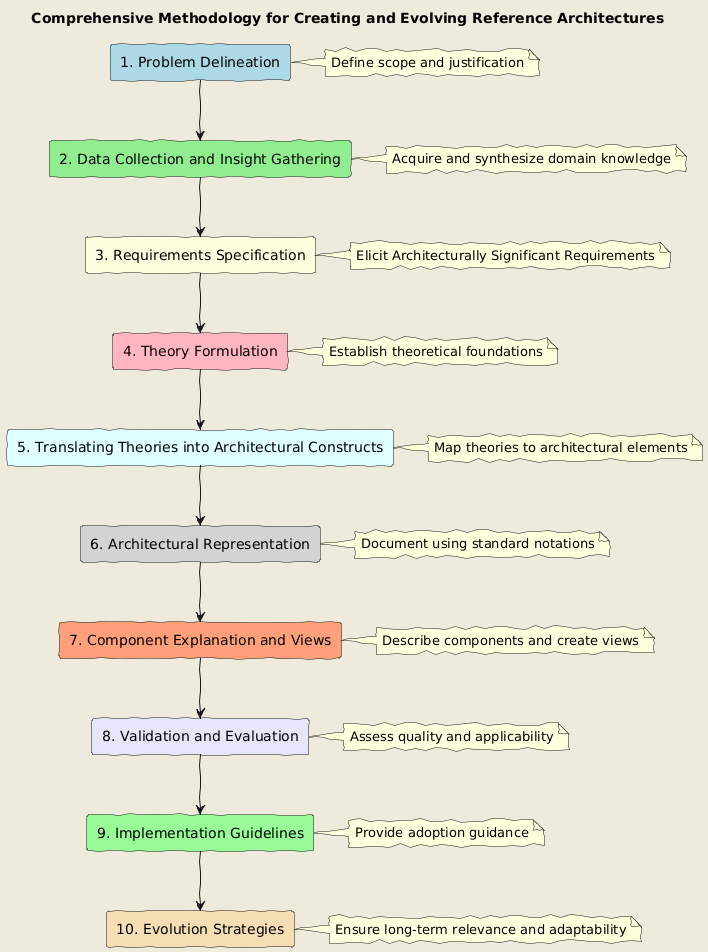
\includegraphics[width=\textwidth]{assets/methodologyPhases.png}

\section{Problem Delineation}
\begin{itemize}
    \item Concept: Defining the scope and justification for the reference architecture
    \item Methods:
    \begin{itemize}
        \item Systematic Literature Review (SLR) to identify gaps and challenges \citep{Kitchenham2004}
        \item Multi-vocal Literature Review to capture practitioner perspectives \citep{Garousi2019}
        \item Stakeholder Analysis to understand diverse architectural needs \citep{Freeman2010}
        \item Case Study Analysis to identify common architectural challenges \citep{Runeson2009}
        \item Gap Analysis to compare existing architectural approaches
        \item Domain-Specific Metrics to quantify potential impact
    \end{itemize}
    \item Outcomes:
    \begin{itemize}
        \item Comprehensive problem statement based on academic and industry evidence
        \item Quantified gaps in existing architectural approaches
        \item Prioritized list of stakeholder needs and challenges
        \item Clear justification for the proposed reference architecture
    \end{itemize}
    \item Alignment with Design Science Research principles \citep{Hevner2004}
    \item Consideration of reference architecture drivers (e.g., standardization, facilitation) \citep{Nakagawa2023}
\end{itemize}


\section{Data Collection and Insight Gathering}
\begin{itemize}
    \item Concept: Comprehensive domain knowledge acquisition and synthesis
    \item Methods:
    \begin{itemize}
        \item Systematic Literature Review (SLR) of academic sources \citep{Kitchenham2007}
        \item Multivocal Literature Review (MLR) of grey literature \citep{Garousi2019}
        \item Semi-structured expert interviews \citep{Bogner2009}
        \item Delphi study for expert consensus on domain challenges \citep{Dalkey1963}
        \item Ethnographic observations of domain practices \citep{Sharp2016}
        \item Survey of domain practitioners \citep{Linaker2015}
    \end{itemize}
    \item Analysis Techniques:
    \begin{itemize}
        \item Thematic analysis of qualitative data \citep{Braun2006}
        \item Grounded theory for emerging concepts \citep{Stol2016}
        \item Cross-case analysis of existing systems \citep{Yin2017}
        \item Domain modeling using feature modeling or ontology engineering \citep{Pohl2005}
    \end{itemize}
    \item Outcomes:
    \begin{itemize}
        \item Comprehensive domain knowledge base
        \item Identified patterns and trends in domain architectures
        \item Catalog of stakeholder concerns and architectural drivers
        \item Domain-specific challenges and opportunities for architectural innovation
    \end{itemize}
    \item Considerations:
    \begin{itemize}
        \item Analysis of existing systems and stakeholder concerns \citep{Nakagawa2023}
        \item Integration of academic and practitioner perspectives
        \item Identification of domain-specific quality attributes and constraints
        \item Mapping of domain concepts to potential architectural elements
    \end{itemize}
\end{itemize}

\section{Requirements Specification}
\begin{itemize}
    \item Concept: Elicitation and documentation of Architecturally Significant Requirements (ASRs) \citep{Chen2013}
    \item Methods:
    \begin{itemize}
        \item Application of ISO/IEC/IEEE 29148:2018 standard \citep{ISO29148}
        \item Quality Attribute Workshops (QAW) to identify key quality attributes \citep{Barbacci2003}
        \item Architecture Business Cycle (ABC) analysis to align with business goals \citep{Bass2003}
        \item Utility Tree construction for prioritizing ASRs \citep{Kazman2000}
        \item Delphi technique for consensus on critical requirements \citep{Dalkey1963}
    \end{itemize}
    \item Outcomes:
    \begin{itemize}
        \item Comprehensive set of ASRs with clear traceability to stakeholder needs
        \item Prioritized list of quality attributes relevant to the reference architecture
        \item Mapping of ASRs to architectural decisions and constraints
    \end{itemize}
    \item Considerations:
    \begin{itemize}
        \item Incorporation of domain-specific standards and regulations \citep{Nakagawa2023}
        \item Analysis of variability in requirements across the domain \citep{Galster2014}
        \item Integration with model-based requirements engineering approaches \citep{Mavin2009}
    \end{itemize}
\end{itemize}



\section{Theory Formulation}
\begin{itemize}
    \item Concept: Establishing theoretical foundations for the reference architecture
    \item Methods:
    \begin{itemize}
        \item Abductive inference for kernel and design theory development \citep{Dubois2014}
        \item Grounded Theory approach for theory building from data \citep{Glaser1967}
        \item Meta-ethnography for synthesizing qualitative studies \citep{Noblit1988}
        \item Design Science Research for developing prescriptive theories \citep{Gregor2013}
    \end{itemize}
    \item Theory Development Process:
    \begin{itemize}
        \item Identification of core concepts and relationships
        \item Formulation of propositions and hypotheses
        \item Development of explanatory and predictive models
        \item Iterative refinement and validation of theories
    \end{itemize}
    \item Theoretical Frameworks to Consider:
    \begin{itemize}
        \item Architectural patterns and styles specific to the domain \citep{Nakagawa2023}
        \item Contingency theory for context-dependent architectural decisions \citep{Kallinikos2006}
        \item Systems theory for understanding complex interactions \citep{Bertalanffy1968}
        \item Socio-technical systems theory for aligning architecture with organizational context \citep{Baxter2011}
    \end{itemize}
    \item Outcomes:
    \begin{itemize}
        \item Kernel theories explaining fundamental domain principles
        \item Design theories guiding architectural decision-making
        \item Theoretical model of the reference architecture
        \item Propositions for empirical validation
    \end{itemize}
    \item Considerations:
    \begin{itemize}
        \item Integration of domain-specific and general architectural theories
        \item Alignment of theories with collected empirical data
        \item Balancing explanatory power with practical applicability
        \item Ensuring theoretical foundations support variability and evolution
    \end{itemize}
\end{itemize}


\section{Translating Theories into Architectural Constructs}
\begin{itemize}
    \item Concept: Systematic translation of theoretical foundations into concrete architectural elements
    \item Methods:
    \begin{itemize}
        \item Theory-to-architecture mapping techniques \citep{Eden2006}
        \item Variability management approaches \citep{Galster2014}
        \item SPES modeling framework for model-based design \citep{Nakagawa2023}
        \item Architecture Description Language (ADL) for formal representation \citep{Medvidovic2000}
        \item Quality Attribute Scenarios for operationalizing quality requirements \citep{Bass2003}
    \end{itemize}
    \item Translation Process:
    \begin{itemize}
        \item Identification of key theoretical concepts and relationships
        \item Mapping of concepts to architectural elements and patterns
        \item Definition of variability points and mechanisms
        \item Formalization of architectural decisions and rationales
        \item Integration of domain-specific constraints and standards
    \end{itemize}
    \item Architectural Constructs to Consider:
    \begin{itemize}
        \item Components, connectors, and their configurations
        \item Architectural styles and patterns relevant to the domain
        \item Variability mechanisms (e.g., parameterization, optional features)
        \item Cross-cutting concerns and their architectural representations
        \item Interfaces and protocols for inter-component communication
    \end{itemize}
    \item Outcomes:
    \begin{itemize}
        \item Comprehensive set of architectural constructs derived from theories
        \item Formal architecture description using selected ADL
        \item Variability model capturing architectural alternatives
        \item Traceability links between theories and architectural elements
        \item Set of architectural tactics addressing quality attributes
    \end{itemize}
    \item Considerations:
    \begin{itemize}
        \item Balancing abstraction and concreteness in architectural representations
        \item Ensuring consistency between theoretical foundations and architectural constructs
        \item Addressing domain-specific requirements and constraints
        \item Facilitating extensibility and evolvability of the reference architecture
        \item Validating the completeness and correctness of the translation
    \end{itemize}
\end{itemize}


\section{Architectural Representation}
\begin{itemize}
    \item Concept: Standardized and comprehensive documentation of the reference architecture
    \item Methods:
    \begin{itemize}
        \item ISO/IEC/IEEE 42010:2011 for architecture description \citep{ISO42010}
        \item ArchiMate for enterprise architecture modeling \citep{Lankhorst2017}
        \item UML and SysML for system and software modeling \citep{OMG2017}
        \item Architecture Description Languages (ADLs) for formal representation \citep{Medvidovic2000}
        \item Domain-specific modeling languages (e.g., AADL for embedded systems) \citep{Feiler2012}
        \item Model-Based Systems Engineering (MBSE) approaches \citep{Estefan2007}
    \end{itemize}
    \item Representation Process:
    \begin{itemize}
        \item Identification of key stakeholders and their concerns \citep{Rozanski2012}
        \item Selection of appropriate viewpoints and views \citep{Kruchten1995}
        \item Definition of architecture elements and their relationships
        \item Specification of interfaces and protocols
        \item Documentation of architectural decisions and rationales \citep{Tyree2005}
        \item Creation of architecture models using selected notations
    \end{itemize}
    \item Representation Aspects to Consider:
    \begin{itemize}
        \item Structural views (e.g., component diagrams, deployment diagrams)
        \item Behavioral views (e.g., sequence diagrams, state machines)
        \item Functional views (e.g., use case diagrams, activity diagrams)
        \item Information views (e.g., data models, information flow diagrams)
        \item Non-functional aspects (e.g., quality attribute scenarios, performance models)
        \item Variability representation (e.g., feature models, variation points) \citep{Galster2014}
    \end{itemize}
    \item Outcomes:
    \begin{itemize}
        \item Comprehensive set of architecture views and models
        \item Formal architecture description using selected ADL or modeling language
        \item Traceability between architectural elements and stakeholder concerns
        \item Documentation of architectural patterns and styles used
        \item Representation of variability and extension points
        \item Alignment with domain-specific standards and best practices
    \end{itemize}
    \item Considerations:
    \begin{itemize}
        \item Balancing detail and abstraction in architectural representations \citep{Maier2009}
        \item Ensuring consistency across different views and models
        \item Addressing domain-specific representation requirements
        \item Facilitating communication among diverse stakeholders
        \item Supporting automated analysis and verification of architectural properties
        \item Enabling integration with model-driven development approaches \citep{Schmidt2006}
        \item Consideration of emerging paradigms (e.g., IoT, Industry 4.0) in representation \citep{Nakagawa2023}
    \end{itemize}
\end{itemize}

\section{Component Explanation and Views}
\begin{itemize}
    \item Concept: Comprehensive architectural description through multiple perspectives
    \item Methods:
    \begin{itemize}
        \item 4+1 View Model of Architecture \citep{Kruchten1995}
        \item Views and Beyond approach \citep{Clements2010}
        \item Viewpoint-oriented systems engineering \citep{Finkelstein1992}
        \item ISO/IEC/IEEE 42010:2011 viewpoint framework \citep{ISO42010}
        \item RAMI 4.0 viewpoints for industrial applications \citep{Adolphs2015}
    \end{itemize}
    \item View Types and Their Purpose:
    \begin{itemize}
        \item Logical view: Functional requirements and system decomposition
        \item Process view: Concurrency and synchronization aspects
        \item Development view: Software management and reuse
        \item Physical view: System topology and distribution
        \item Scenarios: Integrating and validating the four views \citep{Kruchten1995}
        \item Information view: Data models and information flow \citep{Rozanski2012}
        \item Context view: System relationships and dependencies \citep{Rozanski2012}
    \end{itemize}
    \item Component Description Elements:
    \begin{itemize}
        \item Interfaces and protocols
        \item Behavior specifications
        \item Quality attribute characteristics
        \item Variability points and configuration options
        \item Dependencies and constraints
        \item Rationale for design decisions \citep{Tyree2005}
    \end{itemize}
    \item View Integration and Consistency:
    \begin{itemize}
        \item Cross-view traceability techniques \citep{Mader2009}
        \item Consistency checking methods \citep{Egyed2007}
        \item View synchronization strategies \citep{Fradet2008}
    \end{itemize}
    \item Outcomes:
    \begin{itemize}
        \item Comprehensive set of architectural views
        \item Detailed component descriptions with rationales
        \item Traceability between views and stakeholder concerns
        \item Consistency analysis results across views
        \item Integration with domain-specific viewpoints (e.g., RAMI 4.0)
    \end{itemize}
    \item Considerations:
    \begin{itemize}
        \item Tailoring views to specific stakeholder needs \citep{Rozanski2012}
        \item Balancing completeness with understandability
        \item Addressing domain-specific view requirements
        \item Integrating with model-driven approaches \citep{Schmidt2006}
        \item Supporting architectural knowledge management \citep{Farenhorst2007}
        \item Facilitating architecture evaluation through views \citep{Kazman2000}
        \item Consideration of emerging paradigms (e.g., IoT, Industry 4.0) in viewpoint selection \citep{Nakagawa2023}
    \end{itemize}
\end{itemize}

\section{Validation and Evaluation}
\begin{itemize}
    \item Concept: Rigorous quality assessment and validation of the reference architecture
    \item Methods:
    \begin{itemize}
        \item Case studies for real-world application assessment \citep{Runeson2009}
        \item Expert evaluations and surveys \citep{Beecham2005}
        \item Simulation and modeling for performance analysis \citep{Martens2010}
        \item Architecture Tradeoff Analysis Method (ATAM) \citep{Kazman2000}
        \item Scenario-based architecture analysis \citep{Dobrica2002}
        \item Prototype implementation and testing \citep{Gorton2006}
        \item Formal verification techniques \citep{Baier2008}
    \end{itemize}
    \item Evaluation Criteria:
    \begin{itemize}
        \item Functional correctness and completeness
        \item Quality attribute satisfaction (e.g., performance, security, maintainability)
        \item Stakeholder concern coverage
        \item Architectural style and pattern appropriateness
        \item Variability and extensibility support
        \item Compliance with domain-specific standards and regulations \citep{Nakagawa2023}
        \item Interoperability and integration capabilities
    \end{itemize}
    \item Validation Process:
    \begin{itemize}
        \item Definition of validation goals and metrics
        \item Selection of appropriate validation methods
        \item Design and execution of validation experiments
        \item Data collection and analysis
        \item Interpretation of results and feedback incorporation
        \item Iterative refinement of the reference architecture
    \end{itemize}
    \item Outcomes:
    \begin{itemize}
        \item Quantitative and qualitative assessment results
        \item Identified strengths and weaknesses of the reference architecture
        \item Validation reports and documentation
        \item Recommendations for architecture improvements
        \item Confidence level in the architecture's applicability and effectiveness
    \end{itemize}
    \item Considerations:
    \begin{itemize}
        \item Balancing thoroughness of evaluation with time and resource constraints
        \item Addressing domain-specific validation requirements
        \item Ensuring objectivity and reducing bias in expert evaluations
        \item Validating both structural and behavioral aspects of the architecture
        \item Assessing the architecture's ability to meet future domain challenges
        \item Evaluating the architecture's support for emerging technologies and paradigms \citep{Nakagawa2023}
        \item Considering the impact of architectural decisions on system quality attributes \citep{Bass2003}
    \end{itemize}
\end{itemize}

\section{Implementation Guidelines}
\begin{itemize}
    \item Concept: Bridging theory and practice in reference architecture adoption
    \item Methods:
    \begin{itemize}
        \item Detailed guidance based on common implementation challenges \citep{Martínez-Fernández2013}
        \item Architectural instantiation processes \citep{Angelov2012}
        \item Tailoring strategies for specific organizational contexts \citep{Galster2014}
        \item Pattern-based architecture realization \citep{Buschmann2007}
        \item Model-driven architecture implementation approaches \citep{Schmidt2006}
    \end{itemize}
    \item Implementation Process:
    \begin{itemize}
        \item Gap analysis between current and target architecture \citep{Hanschke2010}
        \item Prioritization of implementation activities \citep{Bredemeyer2002}
        \item Incremental adoption strategies \citep{Zimmermann2015}
        \item Customization and extension of reference architecture components \citep{Galster2011}
        \item Integration with existing systems and processes \citep{Lankhorst2017}
    \end{itemize}
    \item Key Considerations:
    \begin{itemize}
        \item Alignment with business goals and stakeholder requirements \citep{Ross2006}
        \item Handling of architectural variability points \citep{Galster2014}
        \item Management of architectural constraints and trade-offs \citep{Bass2003}
        \item Consideration of non-functional requirements in implementation \citep{Chung2012}
        \item Addressing organizational and cultural challenges \citep{Lange2016}
    \end{itemize}
    \item Outcomes:
    \begin{itemize}
        \item Detailed implementation roadmap
        \item Customized reference architecture instances
        \item Set of best practices and lessons learned
        \item Guidelines for architectural governance during implementation
        \item Metrics for measuring implementation success
    \end{itemize}
    \item Challenges and Mitigation Strategies:
    \begin{itemize}
        \item Overcoming resistance to architectural change \citep{Zimmermann2015}
        \item Managing complexity in large-scale implementations \citep{Kruchten2006}
        \item Ensuring consistency across different implementation projects \citep{Clements2010}
        \item Balancing standardization with flexibility \citep{Angelov2012}
        \item Addressing skills gaps and training needs \citep{Martínez-Fernández2013}
    \end{itemize}
    \item Emerging Trends:
    \begin{itemize}
        \item Agile and iterative implementation approaches \citep{Madison2010}
        \item DevOps integration in architecture implementation \citep{Bass2015}
        \item Consideration of emerging technologies (e.g., microservices, containerization) \citep{Newman2015}
        \item Adaptation to Industry 4.0 and IoT paradigms \citep{Nakagawa2023}
    \end{itemize}
\end{itemize}

\section{Evolution Strategies}
\begin{itemize}
    \item Concept: Ensuring long-term relevance and adaptability of the reference architecture
    \item Methods:
    \begin{itemize}
        \item Continuous refinement techniques and adaptation mechanisms \citep{Eixelsberger1998}
        \item Architecture-centric evolution approaches \citep{Garlan2009}
        \item Change impact analysis methods \citep{Lehnert2013}
        \item Version control and configuration management for architectures \citep{Estublier2005}
        \item Architectural knowledge management for evolution support \citep{Farenhorst2007}
    \end{itemize}
    \item Evolution Process:
    \begin{itemize}
        \item Periodic architecture assessments and gap analysis \citep{Kazman2000}
        \item Identification of architectural drift and erosion \citep{Perry1992}
        \item Prioritization of evolution needs based on stakeholder feedback \citep{Bosch2004}
        \item Incremental and iterative architecture updates \citep{Mens2008}
        \item Documentation and communication of architectural changes \citep{Jansen2009}
    \end{itemize}
    \item Key Considerations:
    \begin{itemize}
        \item Balancing stability and flexibility in the architecture \citep{Ozkaya2008}
        \item Managing architectural technical debt \citep{Kruchten2012}
        \item Ensuring backward compatibility during evolution \citep{Garlan2009}
        \item Adapting to emerging technologies and paradigms \citep{Nakagawa2023}
        \item Maintaining traceability between evolving architectural elements \citep{Cleland-Huang2012}
    \end{itemize}
    \item Evolution Strategies:
    \begin{itemize}
        \item Modularization and loose coupling for easier component updates \citep{Baldwin2000}
        \item Design for variability and extensibility \citep{Galster2014}
        \item Use of architectural patterns that support evolution \citep{Buschmann2007}
        \item Adoption of microservices for independent service evolution \citep{Newman2015}
        \item Implementation of feature toggles for gradual feature introduction \citep{Hodgson2017}
    \end{itemize}
    \item Outcomes:
    \begin{itemize}
        \item Evolving reference architecture that remains relevant over time
        \item Documented evolution history and rationale
        \item Set of evolution patterns and best practices
        \item Metrics for measuring architecture evolvability
        \item Reduced architectural technical debt
    \end{itemize}
    \item Challenges and Mitigation:
    \begin{itemize}
        \item Managing complexity during long-term evolution \citep{Kruchten2006}
        \item Balancing short-term needs with long-term architectural integrity \citep{Bosch2004}
        \item Ensuring consistency across different versions of the architecture \citep{Garlan2009}
        \item Addressing resistance to architectural changes \citep{Zimmermann2015}
        \item Maintaining architectural knowledge throughout evolution \citep{Farenhorst2007}
    \end{itemize}
\end{itemize}

\section{Threats to Validity}
\begin{itemize}
    \item Concept: Methodology limitations and potential biases
    \item Method: Systematic identification and mitigation strategies \citep{Wohlin2012}
    \item Optional to consider: Consideration of domain-specific challenges and limitations \citep{Nakagawa2023}
\end{itemize}

\section{Discussion}
\begin{itemize}
    \item Concept: Comparative analysis and potential impact of the proposed methodology
    \item Method: Critical reflection on methodology strengths and limitations
    \item Optional to consider: Discussion on the role of reference architectures in emerging paradigms (e.g., IoT, Industry 4.0) \citep{Nakagawa2023}
\end{itemize}

\section{Conclusion}
\begin{itemize}
    \item Concept: Synthesis of contributions to reference architecture design
    \item Method: Summary of key methodological advancements and future research directions
    \item Optional to consider: Reflection on the future of reference architectures and their role in system development \citep{Nakagawa2023}
\end{itemize}

\bibliographystyle{apalike}
\bibliography{references}

\end{document}